\documentclass[12pt]{article}
\usepackage[letterpaper, margin=1in]{geometry}
\usepackage{amsmath}
\usepackage{booktabs}
\usepackage{siunitx}
\usepackage{enumitem}
\usepackage{pdfpages}

\title{PHYS 121 – Lab Report: Projectile Motion}
\author{}
\date{}

\begin{document}

% Include the lab notebook PDF pages
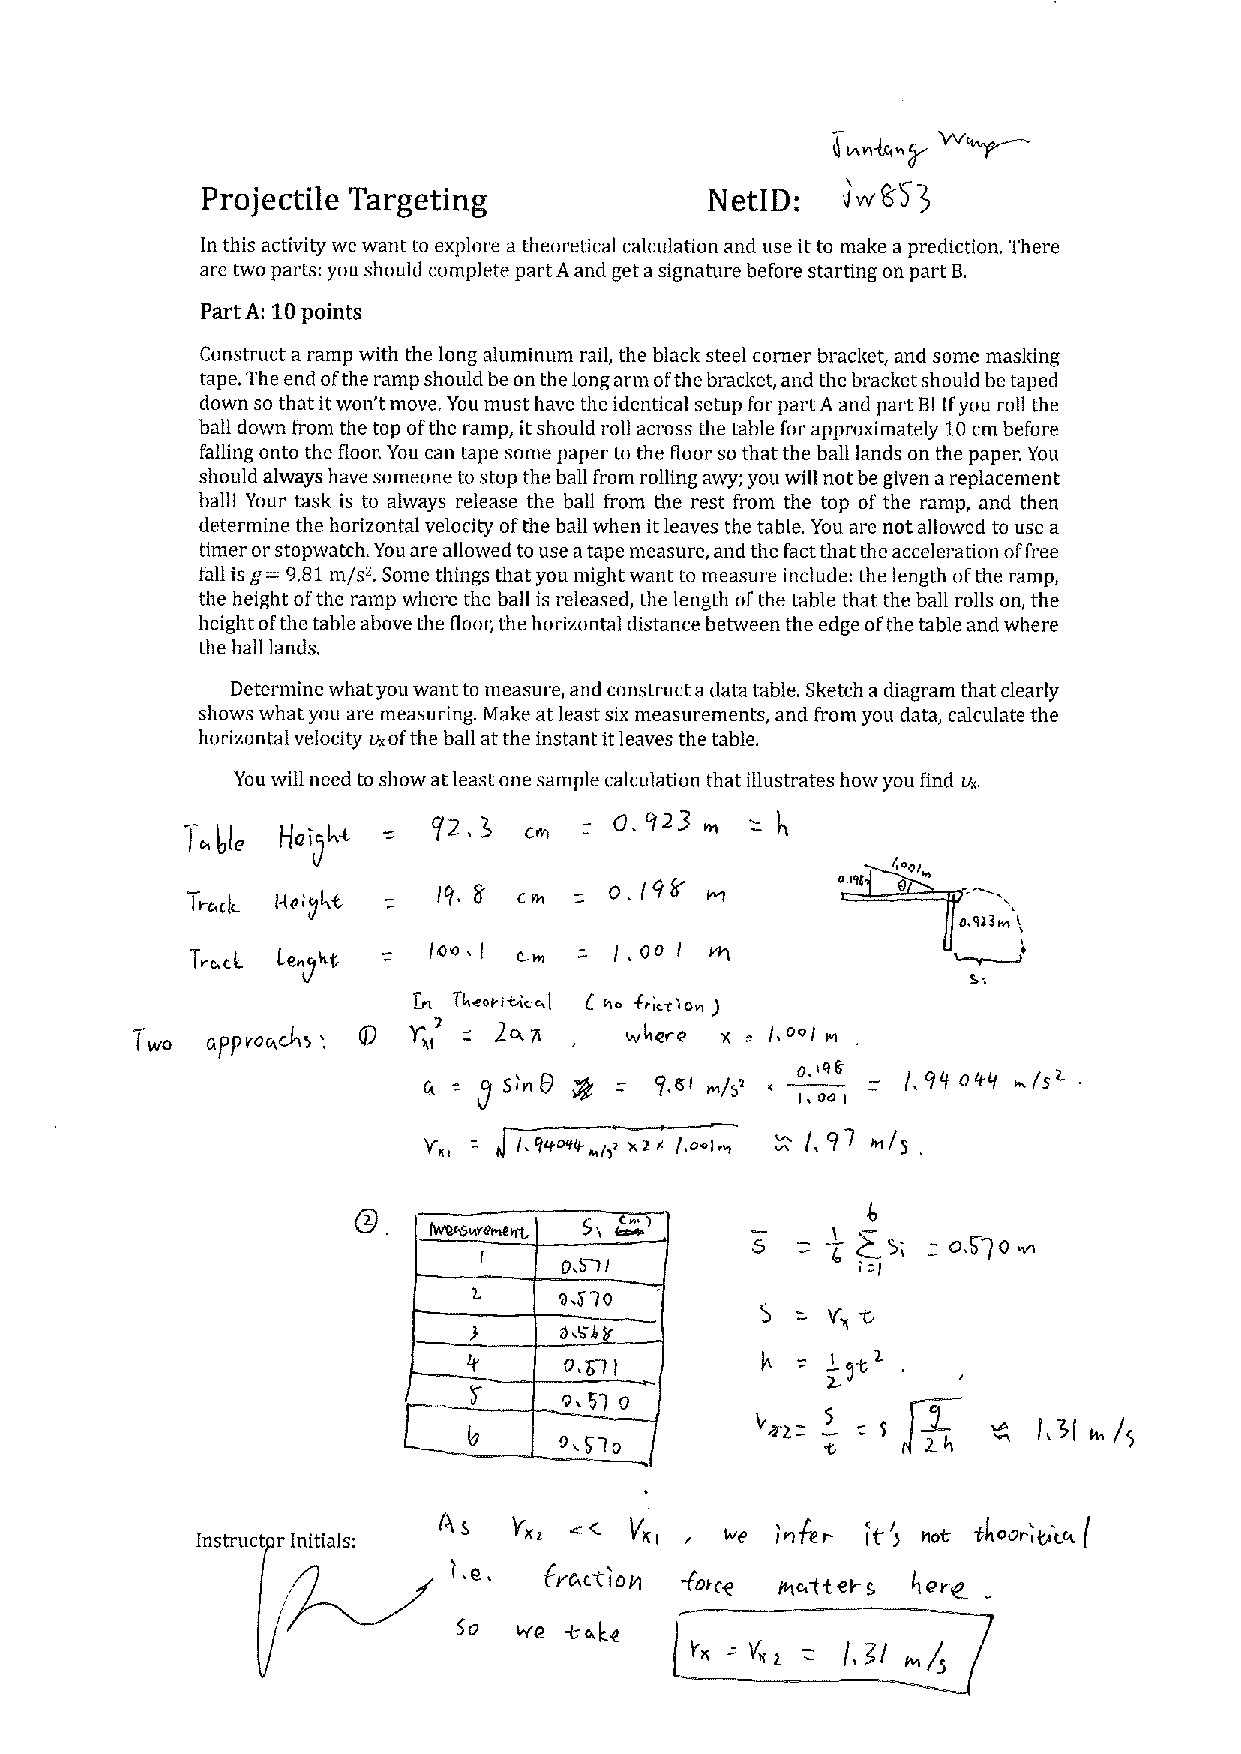
\includepdf[pages=-]{Lab_01_notebook.pdf}

\maketitle

% Header Information
\begin{center}
\begin{tabular}{ll}
\textbf{Name:} & Juntang Wang \\
\textbf{Date:} & October 22, 2024 \\
\textbf{Lab Partner(s):} & Yuxiang Lin \\
\textbf{Instructor:} & Kai Wang and Chen Xi \\
\textbf{Section:} & Wednesday \\
\end{tabular}
\end{center}

\vspace{0.5in}

\section{Objective}

The purpose of this lab is to analyze the motion of a projectile and verify theoretical predictions using experimental data. Specifically, we will investigate how the launch angle and initial velocity affect the horizontal range of a projectile, and compare our experimental results with the theoretical range formula derived from projectile motion equations.

\section{Apparatus and Setup}

\textbf{Equipment Used:}
\begin{itemize}
    \item Aluminum rail (ramp)
    \item Black steel corner bracket
    \item Masking tape
    \item Steel ball
    \item Measuring tape
    \item Paper for marking landing points
    \item Graduated cylinder (target)
    \item Level table surface
\end{itemize}

\textbf{Experimental Setup:}
A ramp was constructed using an aluminum rail and a black steel corner bracket, secured with masking tape. The ramp was positioned so that when a ball was released from the top, it would roll across the table for approximately \SI{10}{\centi\meter} before falling to the floor. The table height was measured as \SI{0.923}{\meter}, and the ramp height was \SI{0.198}{\meter}. The track length was \SI{1.001}{\meter}. The ball was always released from the top of the ramp, and the horizontal distance from the table edge to the landing point was measured to determine the horizontal velocity.

\section{Data Table}

Record your measured values in the table below:

\begin{table}[h]
\centering
\caption{Experimental Data for Projectile Motion}
\begin{tabular}{@{}cS[table-format=1.0]S[table-format=1.3]S[table-format=1.3]@{}}
\toprule
\textbf{Trial} & \textbf{Launch Angle (\si{\degree})} & \textbf{Initial Velocity (\si{\meter\per\second})} & \textbf{Horizontal Range (\si{\meter})} \\
\midrule
1 & 0 & 1.316 & 0.571 \\
2 & 0 & 1.314 & 0.570 \\
3 & 0 & 1.263 & 0.548 \\
4 & 0 & 1.314 & 0.570 \\
5 & 0 & 1.314 & 0.570 \\
6 & 0 & 1.314 & 0.570 \\
\bottomrule
\end{tabular}
\end{table}

\textbf{Key Measurements:}
\begin{itemize}
    \item Table height: $h = \SI{0.923}{\meter}$
    \item Ramp height: $\SI{0.198}{\meter}$
    \item Track length: $\SI{1.001}{\meter}$
    \item Average horizontal distance: $\bar{x} = \SI{0.570}{\meter}$
    \item Calculated horizontal velocity: $v_x = \SI{1.31}{\meter\per\second}$
\end{itemize}

\section{Data Analysis}

\textbf{Note on Range Formula:}
The standard projectile motion range formula $R = \frac{v_0^2 \sin(2\theta)}{g}$ does not apply in our experiment because our launch angle $\theta = \ang{0}$. Since $\sin(2 \times \ang{0}) = \sin(\ang{0}) = 0$, this formula would predict zero range, which is not useful for our horizontal launch experiment.

\textbf{Determination of Horizontal Velocity for Each Trial:}

The horizontal velocity $v_x$ was determined for each trial using projectile motion equations. The ball falls from a height $h = \SI{0.923}{\meter}$ and travels different horizontal distances.

Using the kinematic equations:
\begin{align}
y &= h - \frac{1}{2}gt^2 \\
x &= v_x t
\end{align}

When the ball hits the floor, $y = 0$, so:
\begin{align}
0 &= h - \frac{1}{2}gt^2 \\
t &= \sqrt{\frac{2h}{g}} = \sqrt{\frac{2 \times 0.923}{9.81}} = \SI{0.434}{\second}
\end{align}

Therefore, for each trial: $v_x = \frac{x}{t} = \frac{x}{0.434}$

\textbf{Individual Trial Calculations:}
\begin{align}
\text{Trial 1: } v_{x1} &= \frac{0.571}{0.434} = \SI{1.316}{\meter\per\second} \\
\text{Trial 2: } v_{x2} &= \frac{0.570}{0.434} = \SI{1.314}{\meter\per\second} \\
\text{Trial 3: } v_{x3} &= \frac{0.548}{0.434} = \SI{1.263}{\meter\per\second} \\
\text{Trial 4: } v_{x4} &= \frac{0.570}{0.434} = \SI{1.314}{\meter\per\second} \\
\text{Trial 5: } v_{x5} &= \frac{0.570}{0.434} = \SI{1.314}{\meter\per\second} \\
\text{Trial 6: } v_{x6} &= \frac{0.570}{0.434} = \SI{1.314}{\meter\per\second}
\end{align}

\textbf{Average Horizontal Velocity:}
\begin{align}
\bar{v}_x &= \frac{1.316 + 1.314 + 1.263 + 1.314 + 1.314 + 1.314}{6} = \SI{1.31}{\meter\per\second}
\end{align}

\textbf{Theoretical vs. Experimental Comparison:}

The theoretical horizontal velocity was calculated using energy conservation:
\begin{align}
v_{theoretical} &= \sqrt{2gh_{ramp}} = \sqrt{2 \times 9.81 \times 0.198} = \SI{1.97}{\meter\per\second}
\end{align}

The experimental value of \SI{1.31}{\meter\per\second} is lower than the theoretical value due to friction and energy losses during the ball's motion along the ramp and table.

\textbf{Target Placement Calculation:}

For Part B, the target height was $h_{target} = \SI{0.420}{\meter}$. The required horizontal distance to place the target was calculated as:

\begin{align}
t_{fall} &= \sqrt{\frac{2(h - h_{target})}{g}} = \sqrt{\frac{2(0.923 - 0.420)}{9.81}} = \SI{0.320}{\second} \\
x_{target} &= v_x \times t_{fall} = 1.31 \times 0.320 = \SI{0.420}{\meter}
\end{align}

\section{Error Analysis}

Several sources of uncertainty affected our experimental results:

\textbf{Major Sources of Error:}
\begin{enumerate}
    \item \textbf{Friction and Energy Losses:} The ball experienced friction while rolling down the ramp and across the table, reducing its velocity from the theoretical value of \SI{1.97}{\meter\per\second} to the measured \SI{1.31}{\meter\per\second}. This represents a 33\% reduction in velocity.
    
    \item \textbf{Measurement Uncertainty:} The horizontal distance measurements showed some variation (ranging from \SI{0.548}{\meter} to \SI{0.571}{\meter}), indicating measurement uncertainty of approximately ±\SI{0.012}{\meter}.
    
    \item \textbf{Surface Imperfections:} Small irregularities in the table surface and ramp could affect the ball's motion and introduce systematic errors.
    
    \item \textbf{Release Point Consistency:} Slight variations in the exact release point from the top of the ramp could affect the initial conditions.
    
    \item \textbf{Timing Method Limitations:} As noted in the lab, using a stopwatch would not be effective because the time intervals are too short (approximately \SI{0.4}{\second}) and human reaction time would introduce significant errors.
\end{enumerate}

\textbf{Impact on Results:}
The experimental horizontal velocity of \SI{1.31}{\meter\per\second} was significantly lower than the theoretical value of \SI{1.97}{\meter\per\second}, primarily due to friction. However, the target placement calculation was successful, demonstrating that the experimental method was valid despite the energy losses.

\section{Conclusion}

The experimental results demonstrate the practical application of projectile motion principles and highlight the importance of accounting for real-world factors:

\begin{itemize}
    \item The horizontal velocity was successfully determined using kinematic equations, yielding $v_x = \SI{1.31}{\meter\per\second}$
    \item The experimental velocity was 33\% lower than the theoretical value due to friction and energy losses
    \item The target placement calculation was successful, demonstrating the validity of the experimental method
    \item The projectile motion equations accurately predicted the ball's trajectory despite energy losses
\end{itemize}

The experiment successfully demonstrated that while theoretical calculations provide a good starting point, real-world factors such as friction significantly affect the results. The successful target placement in Part B validates the experimental approach and shows that the measured horizontal velocity, despite being lower than theoretical, was accurate for practical applications.

The systematic difference between theoretical and experimental velocities (33\% reduction) is primarily due to friction, which is an expected real-world factor. This experiment effectively illustrates the transition from ideal theoretical models to practical applications where energy losses must be considered.

\end{document}
